\subsection*{Partie 1 : variations}
\begin{enumerate}
 \item 
\begin{figure}[h!]
 \centering
 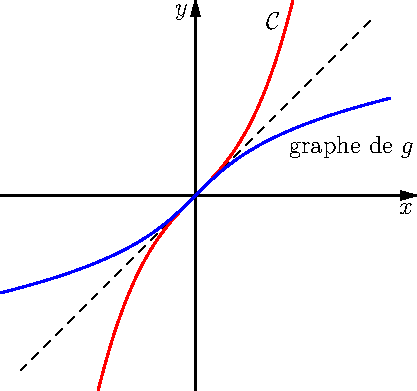
\includegraphics{Capproxrec_1.pdf}
 % Capproxrec_1.pdf: 0x0 pixel, 300dpi, 0.00x0.00 cm, bb=
 \caption{Graphes de $f$ et de $g$.}
 \label{fig:Capproxrec_1}
\end{figure}
La fonction $f$ est croissante comme somme de fonctions croissantes, elle est impaire. Son étude ne présente rien de particulier le graphe est présenté en figure \ref{fig:Capproxrec_1}.
 \item La fonction est strictement croissante donc injective. Elle est continue donc l'image de son domaine de définition $\R$ est un intervalle (théorème des valeurs intermédiaires). Les limites en $+\infty$ et $-\infty$ sont $+\infty$ et $-\infty$ donc cet intervalle image est $\R$. Ceci montre que $f$ est bijective. Sa bijection réciproque est notée $g$. Elle associe à tout réel $x$ l'unique solution de l'équation $t^3+t=x$ d'inconnue $x$. 
 
 \item La bijection réciproque d'une bijection strictement monotone est monotone de même sens. La fonction $g$ est donc strictement croissante.\newline
Pour tout réel $x$, comme $f$ est impaire, $f(-g(x))=-f(g(x))=-x$. Donc $-g(x)$ est l'antécédent de $-x$ ce qui montre que $-g(x)=g(-x)$. La fonction $g$ est donc impaire. Le graphe de $g$ est symétrique de celui de $f$ par rapport à la première bissectrice. Il est placé aussi dans la figure \ref{fig:Capproxrec_1}.

 \item Comme $f'(t)=3t^2+1$, la dérivée $f'$ ne s'annule pas dans $\R$. D'après un théorème de cours, la bijection réciproque $g$ est alors dérivable avec :
\begin{displaymath}
 \forall x\in \R:\; g'(x)=\frac{1}{f'(g(x))}=\frac{1}{1+3g(x)^2}
\end{displaymath}
L'expression de la dérivée de $g$ est clairement positive. De plus, comme $g'$ est strictement croissante, strictement positive dans $]0,+\infty[$ et strictement négative dans $]-\infty, 0 [$, elle est croissante dans $]-\infty,0]$ et décroissante dans $[0,+\infty[$.
\end{enumerate}

\subsection*{Partie 2 : approximations}
\begin{figure}[h!]
 \centering
 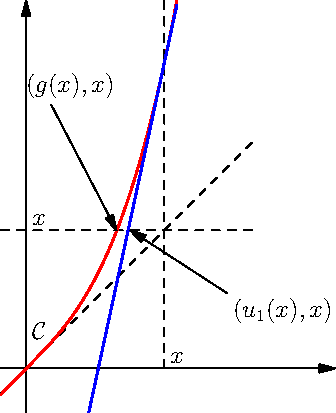
\includegraphics{Capproxrec_2.pdf}
 \caption{Intersection de la tangente avec $D_x$.}
 \label{fig:Capproxrec_2}
\end{figure}
\begin{enumerate}
 \item Notons $X$ et $Y$ les fonctions coordonnées. L'équation de la tangente à $\mathcal C$ au point d'abscisse $t$ est
\begin{displaymath}
 \begin{vmatrix}
  X-t      &  1\\
  Y -t^3-t & 3t^2+1
 \end{vmatrix}
=0
\end{displaymath}
L'abscisse du point d'intersection de la tangente avec $D_x$ est obtenue en prenant $Y=x$ dans l'équation de la tangente.
\begin{multline*}
 (X-t)(3t^2+1)=x-t^3-t\Leftrightarrow X(3t^2+1)=x-t^3-t+3t^3+t=2t^3+x\\
\Leftrightarrow
X=\frac{2t^3+x}{3t^2+1}=\varphi_x(t)
\end{multline*}
Par définition de l'algorithme, le calcul précédent montre que $u_{n+1}(x)=\varphi_x(u_n(x))$. La figure \ref{fig:Capproxrec_2} présente la construction de $u_1(x)$. 

 \item 
\begin{enumerate}
 \item Après réduction au même dénominateur, on obtient :
\begin{displaymath}
 \varphi_x(t)-t = \frac{t^3+t-x}{3t^2+1}
\end{displaymath}
La fonction $t\rightarrow t^3+t-x$ est strictement croissante et s'annule uniquement en $g(x)$. Elle est donc négative avant $g(x)$ et positive après.
 \item Calcul de $\varphi_x'$.
\begin{displaymath}
 \varphi_x'(t)=\frac{6t^2}{3t^2+1}-(2t^3+x)\frac{6t}{(3t^2+1)^2}
=(t^3+t-x)\frac{6t}{(3t^2+1)^2}
\end{displaymath}
On en déduit le tableau suivant
\begin{center}
\renewcommand{\arraystretch}{1.3}
\begin{tabular}{|l|lllllll|}
\hline
 & $-\infty$ &  & $0$ &  & $g(x)$ &  & $+\infty$\\ \hline
$t-\varphi_x(t)$ &  &  & $-$ &  & $0$ & $+$ & \\ \hline
$\varphi_x'(t)$ &  & $+$ & $0$ & $-$ & $0$ & $+$ & \\ \hline
\end{tabular}
\end{center}
\bigskip

 \item Pour un $x>0$ fixé, précisons bien d'abord que $0<g(x)<x$. En effet, la fonction $t\rightarrow t^3+t-x$ est strictement croissante. Elle est strictement négative en $0$ et strictement positive en $x$, le point $g(x)$ où elle s'annule est donc dans l'intervalle ouvert $]0,x[$.\newline
D'après l'étude des signes précédente, $\varphi_x(x)<x$, $\varphi_x(g(x))=g(x)$ et $\varphi_x$ est croissante donc 
\begin{displaymath}
\varphi_x([g(x),x])=[\varphi_x(g(x)),\varphi_x(x)]=[g(x),\varphi_x(x)]\subset[g(x),x] 
\end{displaymath}
Cela traduit bien que $[g(x),x]$ est stable par $\varphi_x$.

 \item Lorsque $t\geq g(x)$, on a déjà prouvé que $t^3+t-x\geq 0$. De plus, pour $t\leq x$, $t-x$ est négatif donc $t^3+t-x\leq t^3$. En utilisant cette majoration dans l'expression factorisée de $\varphi_x'$ déjà trouvée, on obtient :
\begin{displaymath}
 \varphi_x'(t)\leq\frac{6t^4}{(3t^2+1)^2}\leq\frac{6t^4}{(3t^2)^2}=\frac{2}{3}
\end{displaymath}
\end{enumerate}

 \item 
\begin{enumerate}
 \item \`A cause de la stabilité de l'intervalle, tous les $u_n(x)$ sont dans $[g(x),x]$. L'étude des signes a montré que $u_1(x)\leq u_0(x)$. La croissance de $\varphi_x$ dans l'intervalle entraîne que l'inégalité se propage, la suite est donc strictement décroissante. Elle est minorée donc elle converge vers un élément $l$ de l'intervalle. Cette limite $l$ est un point fixe car $\varphi_x$ est continue en $l$. Le seul point fixe dans l'intervalle étant $g(x)$, on en déduit que la suite converge vers $g(x)$. 
 
 \item On sait que tous les $u_n(x)$ sont supérieurs à $g(x)$. Appliquons l'inégalité des accroissements finis à $\varphi_x$ entre $g(x)$ et $u_n(x)$ avec $\frac{2}{3}$ comme majorant de la dérivée dans l'intervalle
\begin{displaymath}
 0\leq u_{n+1}(x)-g(x)=\varphi_x(u_n(x))-\varphi_x(g(x)
\leq (u_n(x)-g(x))\frac{2}{3}
\end{displaymath}

 \item On déduit facilement par récurrence que 
\begin{displaymath}
 u_n(x)-g(x)\leq \left(\frac{2}{3} \right)^n(x-g(x))
\end{displaymath}
 Or lorsque $x$ est plus petit qu'un $a$ fixé, $0\leq x-g(x)\leq x\leq a$. On en déduit $\beta_n\leq\left(\frac{2}{3} \right)^n a$.
 
 \item Développons le numérateur de l'expression proposée à droite de l'égalité puis remplaçons $g(x)^3$ en utilisant $g(x)^3+g(x)=x$. Il vient :
\begin{multline*}
 (t-g(x))^2(2t+g(x))=
2t^3+x-g(x)(3t^2+1)\\
\Rightarrow
(t-g(x))^2\frac{2t+g(x)}{3t^2+1}=\frac{2t^3+x}{3t^2+1}-g(x)=\varphi_x(t)-g(x)
\end{multline*}
Une majoration de $\frac{2t+g(x)}{3t^2+1}$ pour $t\in [g(x),x]$ est demandée. D'abord :
\begin{displaymath}
 g(x)\leq t \Rightarrow \frac{2t+g(x)}{3t^2+1}\leq \frac{3t}{3t^2+1}
\end{displaymath}
Ensuite :
\begin{displaymath}
 \frac{3t}{3t^2+1}=\frac{1}{t+\frac{1}{3t}}
=\frac{1}{\left( \sqrt{t}-\frac{1}{\sqrt{3t}}\right)^2+\frac{2}{\sqrt{3} }}
\leq \frac{\sqrt{3}}{2}
\end{displaymath}
\end{enumerate}
Ce qui entraîne l'inégalité demandée.
\end{enumerate}
